\documentclass[12pt]{article}
\usepackage{tocloft}
\usepackage{natbib}
\usepackage{float}
\usepackage{url}
\usepackage[utf8x]{inputenc}
\usepackage{amsmath}
\usepackage{graphicx}
\usepackage{verbatim}
\graphicspath{{images/}}
\usepackage{parskip}
\usepackage{fancyhdr}
\usepackage{vmargin}
\setmarginsrb{3 cm}{2.5 cm}{3 cm}{2.5 cm}{1 cm}{1.5 cm}{1 cm}{1.5 cm}
\usepackage{appendix}
\usepackage{listings} % For code importing
\usepackage{xcolor} % for setting colors
 %%%%%%%%%%%%%%%%%%%%%%%%%%%%%%%%%%%%%%%%%%%%%%%%%%%%%%%%%%%%%%%%%%%%%%%%%%%%%%%% 
%%% ~ Arduino Language - Arduino IDE Colors ~                                  %%%
%%%                                                                            %%%
%%% Kyle Rocha-Brownell | 10/2/2017 | No Licence                               %%%
%%% -------------------------------------------------------------------------- %%%
%%%                                                                            %%%
%%% Place this file in your working directory (next to the latex file you're   %%%
%%% working on).  To add it to your project, place:                            %%%
%%%     %%%%%%%%%%%%%%%%%%%%%%%%%%%%%%%%%%%%%%%%%%%%%%%%%%%%%%%%%%%%%%%%%%%%%%%%%%%%%%%% 
%%% ~ Arduino Language - Arduino IDE Colors ~                                  %%%
%%%                                                                            %%%
%%% Kyle Rocha-Brownell | 10/2/2017 | No Licence                               %%%
%%% -------------------------------------------------------------------------- %%%
%%%                                                                            %%%
%%% Place this file in your working directory (next to the latex file you're   %%%
%%% working on).  To add it to your project, place:                            %%%
%%%     %%%%%%%%%%%%%%%%%%%%%%%%%%%%%%%%%%%%%%%%%%%%%%%%%%%%%%%%%%%%%%%%%%%%%%%%%%%%%%%% 
%%% ~ Arduino Language - Arduino IDE Colors ~                                  %%%
%%%                                                                            %%%
%%% Kyle Rocha-Brownell | 10/2/2017 | No Licence                               %%%
%%% -------------------------------------------------------------------------- %%%
%%%                                                                            %%%
%%% Place this file in your working directory (next to the latex file you're   %%%
%%% working on).  To add it to your project, place:                            %%%
%%%    \input{arduinoLanguage.tex}                                             %%%
%%% somewhere before \begin{document} in your latex file.                      %%%
%%%                                                                            %%%
%%% In your document, place your arduino code between:                         %%%
%%%   \begin{lstlisting}[language=Arduino]                                     %%%
%%% and:                                                                       %%%
%%%   \end{lstlisting}                                                         %%%
%%%                                                                            %%%
%%% Or create your own style to add non-built-in functions and variables.      %%%
%%%                                                                            %%%
 %%%%%%%%%%%%%%%%%%%%%%%%%%%%%%%%%%%%%%%%%%%%%%%%%%%%%%%%%%%%%%%%%%%%%%%%%%%%%%%% 

\usepackage{color}
\usepackage{listings}    
\usepackage{courier}

%%% Define Custom IDE Colors %%%
\definecolor{arduinoGreen}    {rgb} {0.17, 0.43, 0.01}
\definecolor{arduinoGrey}     {rgb} {0.47, 0.47, 0.33}
\definecolor{arduinoOrange}   {rgb} {0.8 , 0.4 , 0   }
\definecolor{arduinoBlue}     {rgb} {0.01, 0.61, 0.98}
\definecolor{arduinoDarkBlue} {rgb} {0.0 , 0.2 , 0.5 }

%%% Define Arduino Language %%%
\lstdefinelanguage{Arduino}{
  language=C++, % begin with default C++ settings 
%
%
  %%% Keyword Color Group 1 %%%  (called KEYWORD3 by arduino)
  keywordstyle=\color{arduinoGreen},   
  deletekeywords={  % remove all arduino keywords that might be in c++
                break, case, override, final, continue, default, do, else, for, 
                if, return, goto, switch, throw, try, while, setup, loop, export, 
                not, or, and, xor, include, define, elif, else, error, if, ifdef, 
                ifndef, pragma, warning,
                HIGH, LOW, INPUT, INPUT_PULLUP, OUTPUT, DEC, BIN, HEX, OCT, PI, 
                HALF_PI, TWO_PI, LSBFIRST, MSBFIRST, CHANGE, FALLING, RISING, 
                DEFAULT, EXTERNAL, INTERNAL, INTERNAL1V1, INTERNAL2V56, LED_BUILTIN, 
                LED_BUILTIN_RX, LED_BUILTIN_TX, DIGITAL_MESSAGE, FIRMATA_STRING, 
                ANALOG_MESSAGE, REPORT_DIGITAL, REPORT_ANALOG, SET_PIN_MODE, 
                SYSTEM_RESET, SYSEX_START, auto, int8_t, int16_t, int32_t, int64_t, 
                uint8_t, uint16_t, uint32_t, uint64_t, char16_t, char32_t, operator, 
                enum, delete, bool, boolean, byte, char, const, false, float, double, 
                null, NULL, int, long, new, private, protected, public, short, 
                signed, static, volatile, String, void, true, unsigned, word, array, 
                sizeof, dynamic_cast, typedef, const_cast, struct, static_cast, union, 
                friend, extern, class, reinterpret_cast, register, explicit, inline, 
                _Bool, complex, _Complex, _Imaginary, atomic_bool, atomic_char, 
                atomic_schar, atomic_uchar, atomic_short, atomic_ushort, atomic_int, 
                atomic_uint, atomic_long, atomic_ulong, atomic_llong, atomic_ullong, 
                virtual, PROGMEM,
                Serial, Serial1, Serial2, Serial3, SerialUSB, Keyboard, Mouse,
                abs, acos, asin, atan, atan2, ceil, constrain, cos, degrees, exp, 
                floor, log, map, max, min, radians, random, randomSeed, round, sin, 
                sq, sqrt, tan, pow, bitRead, bitWrite, bitSet, bitClear, bit, 
                highByte, lowByte, analogReference, analogRead, 
                analogReadResolution, analogWrite, analogWriteResolution, 
                attachInterrupt, detachInterrupt, digitalPinToInterrupt, delay, 
                delayMicroseconds, digitalWrite, digitalRead, interrupts, millis, 
                micros, noInterrupts, noTone, pinMode, pulseIn, pulseInLong, shiftIn, 
                shiftOut, tone, yield, Stream, begin, end, peek, read, print, 
                println, available, availableForWrite, flush, setTimeout, find, 
                findUntil, parseInt, parseFloat, readBytes, readBytesUntil, readString, 
                readStringUntil, trim, toUpperCase, toLowerCase, charAt, compareTo, 
                concat, endsWith, startsWith, equals, equalsIgnoreCase, getBytes, 
                indexOf, lastIndexOf, length, replace, setCharAt, substring, 
                toCharArray, toInt, press, release, releaseAll, accept, click, move, 
                isPressed, isAlphaNumeric, isAlpha, isAscii, isWhitespace, isControl, 
                isDigit, isGraph, isLowerCase, isPrintable, isPunct, isSpace, 
                isUpperCase, isHexadecimalDigit, 
                }, 
  morekeywords={   % add arduino structures to group 1
                break, case, override, final, continue, default, do, else, for, 
                if, return, goto, switch, throw, try, while, setup, loop, export, 
                not, or, and, xor, include, define, elif, else, error, if, ifdef, 
                ifndef, pragma, warning,
                }, 
% 
%
  %%% Keyword Color Group 2 %%%  (called LITERAL1 by arduino)
  keywordstyle=[2]\color{arduinoBlue},   
  keywords=[2]{   % add variables and dataTypes as 2nd group  
                HIGH, LOW, INPUT, INPUT_PULLUP, OUTPUT, DEC, BIN, HEX, OCT, PI, 
                HALF_PI, TWO_PI, LSBFIRST, MSBFIRST, CHANGE, FALLING, RISING, 
                DEFAULT, EXTERNAL, INTERNAL, INTERNAL1V1, INTERNAL2V56, LED_BUILTIN, 
                LED_BUILTIN_RX, LED_BUILTIN_TX, DIGITAL_MESSAGE, FIRMATA_STRING, 
                ANALOG_MESSAGE, REPORT_DIGITAL, REPORT_ANALOG, SET_PIN_MODE, 
                SYSTEM_RESET, SYSEX_START, auto, int8_t, int16_t, int32_t, int64_t, 
                uint8_t, uint16_t, uint32_t, uint64_t, char16_t, char32_t, operator, 
                enum, delete, bool, boolean, byte, char, const, false, float, double, 
                null, NULL, int, long, new, private, protected, public, short, 
                signed, static, volatile, String, void, true, unsigned, word, array, 
                sizeof, dynamic_cast, typedef, const_cast, struct, static_cast, union, 
                friend, extern, class, reinterpret_cast, register, explicit, inline, 
                _Bool, complex, _Complex, _Imaginary, atomic_bool, atomic_char, 
                atomic_schar, atomic_uchar, atomic_short, atomic_ushort, atomic_int, 
                atomic_uint, atomic_long, atomic_ulong, atomic_llong, atomic_ullong, 
                virtual, PROGMEM,
                },  
% 
%
  %%% Keyword Color Group 3 %%%  (called KEYWORD1 by arduino)
  keywordstyle=[3]\bfseries\color{arduinoOrange},
  keywords=[3]{  % add built-in functions as a 3rd group
                Serial, Serial1, Serial2, Serial3, SerialUSB, Keyboard, Mouse,
                },      
%
%
  %%% Keyword Color Group 4 %%%  (called KEYWORD2 by arduino)
  keywordstyle=[4]\color{arduinoOrange},
  keywords=[4]{  % add more built-in functions as a 4th group
                abs, acos, asin, atan, atan2, ceil, constrain, cos, degrees, exp, 
                floor, log, map, max, min, radians, random, randomSeed, round, sin, 
                sq, sqrt, tan, pow, bitRead, bitWrite, bitSet, bitClear, bit, 
                highByte, lowByte, analogReference, analogRead, 
                analogReadResolution, analogWrite, analogWriteResolution, 
                attachInterrupt, detachInterrupt, digitalPinToInterrupt, delay, 
                delayMicroseconds, digitalWrite, digitalRead, interrupts, millis, 
                micros, noInterrupts, noTone, pinMode, pulseIn, pulseInLong, shiftIn, 
                shiftOut, tone, yield, Stream, begin, end, peek, read, print, 
                println, available, availableForWrite, flush, setTimeout, find, 
                findUntil, parseInt, parseFloat, readBytes, readBytesUntil, readString, 
                readStringUntil, trim, toUpperCase, toLowerCase, charAt, compareTo, 
                concat, endsWith, startsWith, equals, equalsIgnoreCase, getBytes, 
                indexOf, lastIndexOf, length, replace, setCharAt, substring, 
                toCharArray, toInt, press, release, releaseAll, accept, click, move, 
                isPressed, isAlphaNumeric, isAlpha, isAscii, isWhitespace, isControl, 
                isDigit, isGraph, isLowerCase, isPrintable, isPunct, isSpace, 
                isUpperCase, isHexadecimalDigit, 
                },      
%
%
  %%% Set Other Colors %%%
  stringstyle=\color{arduinoDarkBlue},    
  commentstyle=\color{arduinoGrey},    
%          
%   
  %%%% Line Numbering %%%%
   numbers=left,                    
  numbersep=5pt,                   
  numberstyle=\color{arduinoGrey},    
  %stepnumber=2,                      % show every 2 line numbers
%
%
  %%%% Code Box Style %%%%
  breaklines=true,                    % wordwrapping
  tabsize=2,         
  basicstyle=\ttfamily  
}                                             %%%
%%% somewhere before \begin{document} in your latex file.                      %%%
%%%                                                                            %%%
%%% In your document, place your arduino code between:                         %%%
%%%   \begin{lstlisting}[language=Arduino]                                     %%%
%%% and:                                                                       %%%
%%%   \end{lstlisting}                                                         %%%
%%%                                                                            %%%
%%% Or create your own style to add non-built-in functions and variables.      %%%
%%%                                                                            %%%
 %%%%%%%%%%%%%%%%%%%%%%%%%%%%%%%%%%%%%%%%%%%%%%%%%%%%%%%%%%%%%%%%%%%%%%%%%%%%%%%% 

\usepackage{color}
\usepackage{listings}    
\usepackage{courier}

%%% Define Custom IDE Colors %%%
\definecolor{arduinoGreen}    {rgb} {0.17, 0.43, 0.01}
\definecolor{arduinoGrey}     {rgb} {0.47, 0.47, 0.33}
\definecolor{arduinoOrange}   {rgb} {0.8 , 0.4 , 0   }
\definecolor{arduinoBlue}     {rgb} {0.01, 0.61, 0.98}
\definecolor{arduinoDarkBlue} {rgb} {0.0 , 0.2 , 0.5 }

%%% Define Arduino Language %%%
\lstdefinelanguage{Arduino}{
  language=C++, % begin with default C++ settings 
%
%
  %%% Keyword Color Group 1 %%%  (called KEYWORD3 by arduino)
  keywordstyle=\color{arduinoGreen},   
  deletekeywords={  % remove all arduino keywords that might be in c++
                break, case, override, final, continue, default, do, else, for, 
                if, return, goto, switch, throw, try, while, setup, loop, export, 
                not, or, and, xor, include, define, elif, else, error, if, ifdef, 
                ifndef, pragma, warning,
                HIGH, LOW, INPUT, INPUT_PULLUP, OUTPUT, DEC, BIN, HEX, OCT, PI, 
                HALF_PI, TWO_PI, LSBFIRST, MSBFIRST, CHANGE, FALLING, RISING, 
                DEFAULT, EXTERNAL, INTERNAL, INTERNAL1V1, INTERNAL2V56, LED_BUILTIN, 
                LED_BUILTIN_RX, LED_BUILTIN_TX, DIGITAL_MESSAGE, FIRMATA_STRING, 
                ANALOG_MESSAGE, REPORT_DIGITAL, REPORT_ANALOG, SET_PIN_MODE, 
                SYSTEM_RESET, SYSEX_START, auto, int8_t, int16_t, int32_t, int64_t, 
                uint8_t, uint16_t, uint32_t, uint64_t, char16_t, char32_t, operator, 
                enum, delete, bool, boolean, byte, char, const, false, float, double, 
                null, NULL, int, long, new, private, protected, public, short, 
                signed, static, volatile, String, void, true, unsigned, word, array, 
                sizeof, dynamic_cast, typedef, const_cast, struct, static_cast, union, 
                friend, extern, class, reinterpret_cast, register, explicit, inline, 
                _Bool, complex, _Complex, _Imaginary, atomic_bool, atomic_char, 
                atomic_schar, atomic_uchar, atomic_short, atomic_ushort, atomic_int, 
                atomic_uint, atomic_long, atomic_ulong, atomic_llong, atomic_ullong, 
                virtual, PROGMEM,
                Serial, Serial1, Serial2, Serial3, SerialUSB, Keyboard, Mouse,
                abs, acos, asin, atan, atan2, ceil, constrain, cos, degrees, exp, 
                floor, log, map, max, min, radians, random, randomSeed, round, sin, 
                sq, sqrt, tan, pow, bitRead, bitWrite, bitSet, bitClear, bit, 
                highByte, lowByte, analogReference, analogRead, 
                analogReadResolution, analogWrite, analogWriteResolution, 
                attachInterrupt, detachInterrupt, digitalPinToInterrupt, delay, 
                delayMicroseconds, digitalWrite, digitalRead, interrupts, millis, 
                micros, noInterrupts, noTone, pinMode, pulseIn, pulseInLong, shiftIn, 
                shiftOut, tone, yield, Stream, begin, end, peek, read, print, 
                println, available, availableForWrite, flush, setTimeout, find, 
                findUntil, parseInt, parseFloat, readBytes, readBytesUntil, readString, 
                readStringUntil, trim, toUpperCase, toLowerCase, charAt, compareTo, 
                concat, endsWith, startsWith, equals, equalsIgnoreCase, getBytes, 
                indexOf, lastIndexOf, length, replace, setCharAt, substring, 
                toCharArray, toInt, press, release, releaseAll, accept, click, move, 
                isPressed, isAlphaNumeric, isAlpha, isAscii, isWhitespace, isControl, 
                isDigit, isGraph, isLowerCase, isPrintable, isPunct, isSpace, 
                isUpperCase, isHexadecimalDigit, 
                }, 
  morekeywords={   % add arduino structures to group 1
                break, case, override, final, continue, default, do, else, for, 
                if, return, goto, switch, throw, try, while, setup, loop, export, 
                not, or, and, xor, include, define, elif, else, error, if, ifdef, 
                ifndef, pragma, warning,
                }, 
% 
%
  %%% Keyword Color Group 2 %%%  (called LITERAL1 by arduino)
  keywordstyle=[2]\color{arduinoBlue},   
  keywords=[2]{   % add variables and dataTypes as 2nd group  
                HIGH, LOW, INPUT, INPUT_PULLUP, OUTPUT, DEC, BIN, HEX, OCT, PI, 
                HALF_PI, TWO_PI, LSBFIRST, MSBFIRST, CHANGE, FALLING, RISING, 
                DEFAULT, EXTERNAL, INTERNAL, INTERNAL1V1, INTERNAL2V56, LED_BUILTIN, 
                LED_BUILTIN_RX, LED_BUILTIN_TX, DIGITAL_MESSAGE, FIRMATA_STRING, 
                ANALOG_MESSAGE, REPORT_DIGITAL, REPORT_ANALOG, SET_PIN_MODE, 
                SYSTEM_RESET, SYSEX_START, auto, int8_t, int16_t, int32_t, int64_t, 
                uint8_t, uint16_t, uint32_t, uint64_t, char16_t, char32_t, operator, 
                enum, delete, bool, boolean, byte, char, const, false, float, double, 
                null, NULL, int, long, new, private, protected, public, short, 
                signed, static, volatile, String, void, true, unsigned, word, array, 
                sizeof, dynamic_cast, typedef, const_cast, struct, static_cast, union, 
                friend, extern, class, reinterpret_cast, register, explicit, inline, 
                _Bool, complex, _Complex, _Imaginary, atomic_bool, atomic_char, 
                atomic_schar, atomic_uchar, atomic_short, atomic_ushort, atomic_int, 
                atomic_uint, atomic_long, atomic_ulong, atomic_llong, atomic_ullong, 
                virtual, PROGMEM,
                },  
% 
%
  %%% Keyword Color Group 3 %%%  (called KEYWORD1 by arduino)
  keywordstyle=[3]\bfseries\color{arduinoOrange},
  keywords=[3]{  % add built-in functions as a 3rd group
                Serial, Serial1, Serial2, Serial3, SerialUSB, Keyboard, Mouse,
                },      
%
%
  %%% Keyword Color Group 4 %%%  (called KEYWORD2 by arduino)
  keywordstyle=[4]\color{arduinoOrange},
  keywords=[4]{  % add more built-in functions as a 4th group
                abs, acos, asin, atan, atan2, ceil, constrain, cos, degrees, exp, 
                floor, log, map, max, min, radians, random, randomSeed, round, sin, 
                sq, sqrt, tan, pow, bitRead, bitWrite, bitSet, bitClear, bit, 
                highByte, lowByte, analogReference, analogRead, 
                analogReadResolution, analogWrite, analogWriteResolution, 
                attachInterrupt, detachInterrupt, digitalPinToInterrupt, delay, 
                delayMicroseconds, digitalWrite, digitalRead, interrupts, millis, 
                micros, noInterrupts, noTone, pinMode, pulseIn, pulseInLong, shiftIn, 
                shiftOut, tone, yield, Stream, begin, end, peek, read, print, 
                println, available, availableForWrite, flush, setTimeout, find, 
                findUntil, parseInt, parseFloat, readBytes, readBytesUntil, readString, 
                readStringUntil, trim, toUpperCase, toLowerCase, charAt, compareTo, 
                concat, endsWith, startsWith, equals, equalsIgnoreCase, getBytes, 
                indexOf, lastIndexOf, length, replace, setCharAt, substring, 
                toCharArray, toInt, press, release, releaseAll, accept, click, move, 
                isPressed, isAlphaNumeric, isAlpha, isAscii, isWhitespace, isControl, 
                isDigit, isGraph, isLowerCase, isPrintable, isPunct, isSpace, 
                isUpperCase, isHexadecimalDigit, 
                },      
%
%
  %%% Set Other Colors %%%
  stringstyle=\color{arduinoDarkBlue},    
  commentstyle=\color{arduinoGrey},    
%          
%   
  %%%% Line Numbering %%%%
   numbers=left,                    
  numbersep=5pt,                   
  numberstyle=\color{arduinoGrey},    
  %stepnumber=2,                      % show every 2 line numbers
%
%
  %%%% Code Box Style %%%%
  breaklines=true,                    % wordwrapping
  tabsize=2,         
  basicstyle=\ttfamily  
}                                             %%%
%%% somewhere before \begin{document} in your latex file.                      %%%
%%%                                                                            %%%
%%% In your document, place your arduino code between:                         %%%
%%%   \begin{lstlisting}[language=Arduino]                                     %%%
%%% and:                                                                       %%%
%%%   \end{lstlisting}                                                         %%%
%%%                                                                            %%%
%%% Or create your own style to add non-built-in functions and variables.      %%%
%%%                                                                            %%%
 %%%%%%%%%%%%%%%%%%%%%%%%%%%%%%%%%%%%%%%%%%%%%%%%%%%%%%%%%%%%%%%%%%%%%%%%%%%%%%%% 

\usepackage{color}
\usepackage{listings}    
\usepackage{courier}

%%% Define Custom IDE Colors %%%
\definecolor{arduinoGreen}    {rgb} {0.17, 0.43, 0.01}
\definecolor{arduinoGrey}     {rgb} {0.47, 0.47, 0.33}
\definecolor{arduinoOrange}   {rgb} {0.8 , 0.4 , 0   }
\definecolor{arduinoBlue}     {rgb} {0.01, 0.61, 0.98}
\definecolor{arduinoDarkBlue} {rgb} {0.0 , 0.2 , 0.5 }

%%% Define Arduino Language %%%
\lstdefinelanguage{Arduino}{
  language=C++, % begin with default C++ settings 
%
%
  %%% Keyword Color Group 1 %%%  (called KEYWORD3 by arduino)
  keywordstyle=\color{arduinoGreen},   
  deletekeywords={  % remove all arduino keywords that might be in c++
                break, case, override, final, continue, default, do, else, for, 
                if, return, goto, switch, throw, try, while, setup, loop, export, 
                not, or, and, xor, include, define, elif, else, error, if, ifdef, 
                ifndef, pragma, warning,
                HIGH, LOW, INPUT, INPUT_PULLUP, OUTPUT, DEC, BIN, HEX, OCT, PI, 
                HALF_PI, TWO_PI, LSBFIRST, MSBFIRST, CHANGE, FALLING, RISING, 
                DEFAULT, EXTERNAL, INTERNAL, INTERNAL1V1, INTERNAL2V56, LED_BUILTIN, 
                LED_BUILTIN_RX, LED_BUILTIN_TX, DIGITAL_MESSAGE, FIRMATA_STRING, 
                ANALOG_MESSAGE, REPORT_DIGITAL, REPORT_ANALOG, SET_PIN_MODE, 
                SYSTEM_RESET, SYSEX_START, auto, int8_t, int16_t, int32_t, int64_t, 
                uint8_t, uint16_t, uint32_t, uint64_t, char16_t, char32_t, operator, 
                enum, delete, bool, boolean, byte, char, const, false, float, double, 
                null, NULL, int, long, new, private, protected, public, short, 
                signed, static, volatile, String, void, true, unsigned, word, array, 
                sizeof, dynamic_cast, typedef, const_cast, struct, static_cast, union, 
                friend, extern, class, reinterpret_cast, register, explicit, inline, 
                _Bool, complex, _Complex, _Imaginary, atomic_bool, atomic_char, 
                atomic_schar, atomic_uchar, atomic_short, atomic_ushort, atomic_int, 
                atomic_uint, atomic_long, atomic_ulong, atomic_llong, atomic_ullong, 
                virtual, PROGMEM,
                Serial, Serial1, Serial2, Serial3, SerialUSB, Keyboard, Mouse,
                abs, acos, asin, atan, atan2, ceil, constrain, cos, degrees, exp, 
                floor, log, map, max, min, radians, random, randomSeed, round, sin, 
                sq, sqrt, tan, pow, bitRead, bitWrite, bitSet, bitClear, bit, 
                highByte, lowByte, analogReference, analogRead, 
                analogReadResolution, analogWrite, analogWriteResolution, 
                attachInterrupt, detachInterrupt, digitalPinToInterrupt, delay, 
                delayMicroseconds, digitalWrite, digitalRead, interrupts, millis, 
                micros, noInterrupts, noTone, pinMode, pulseIn, pulseInLong, shiftIn, 
                shiftOut, tone, yield, Stream, begin, end, peek, read, print, 
                println, available, availableForWrite, flush, setTimeout, find, 
                findUntil, parseInt, parseFloat, readBytes, readBytesUntil, readString, 
                readStringUntil, trim, toUpperCase, toLowerCase, charAt, compareTo, 
                concat, endsWith, startsWith, equals, equalsIgnoreCase, getBytes, 
                indexOf, lastIndexOf, length, replace, setCharAt, substring, 
                toCharArray, toInt, press, release, releaseAll, accept, click, move, 
                isPressed, isAlphaNumeric, isAlpha, isAscii, isWhitespace, isControl, 
                isDigit, isGraph, isLowerCase, isPrintable, isPunct, isSpace, 
                isUpperCase, isHexadecimalDigit, 
                }, 
  morekeywords={   % add arduino structures to group 1
                break, case, override, final, continue, default, do, else, for, 
                if, return, goto, switch, throw, try, while, setup, loop, export, 
                not, or, and, xor, include, define, elif, else, error, if, ifdef, 
                ifndef, pragma, warning,
                }, 
% 
%
  %%% Keyword Color Group 2 %%%  (called LITERAL1 by arduino)
  keywordstyle=[2]\color{arduinoBlue},   
  keywords=[2]{   % add variables and dataTypes as 2nd group  
                HIGH, LOW, INPUT, INPUT_PULLUP, OUTPUT, DEC, BIN, HEX, OCT, PI, 
                HALF_PI, TWO_PI, LSBFIRST, MSBFIRST, CHANGE, FALLING, RISING, 
                DEFAULT, EXTERNAL, INTERNAL, INTERNAL1V1, INTERNAL2V56, LED_BUILTIN, 
                LED_BUILTIN_RX, LED_BUILTIN_TX, DIGITAL_MESSAGE, FIRMATA_STRING, 
                ANALOG_MESSAGE, REPORT_DIGITAL, REPORT_ANALOG, SET_PIN_MODE, 
                SYSTEM_RESET, SYSEX_START, auto, int8_t, int16_t, int32_t, int64_t, 
                uint8_t, uint16_t, uint32_t, uint64_t, char16_t, char32_t, operator, 
                enum, delete, bool, boolean, byte, char, const, false, float, double, 
                null, NULL, int, long, new, private, protected, public, short, 
                signed, static, volatile, String, void, true, unsigned, word, array, 
                sizeof, dynamic_cast, typedef, const_cast, struct, static_cast, union, 
                friend, extern, class, reinterpret_cast, register, explicit, inline, 
                _Bool, complex, _Complex, _Imaginary, atomic_bool, atomic_char, 
                atomic_schar, atomic_uchar, atomic_short, atomic_ushort, atomic_int, 
                atomic_uint, atomic_long, atomic_ulong, atomic_llong, atomic_ullong, 
                virtual, PROGMEM,
                },  
% 
%
  %%% Keyword Color Group 3 %%%  (called KEYWORD1 by arduino)
  keywordstyle=[3]\bfseries\color{arduinoOrange},
  keywords=[3]{  % add built-in functions as a 3rd group
                Serial, Serial1, Serial2, Serial3, SerialUSB, Keyboard, Mouse,
                },      
%
%
  %%% Keyword Color Group 4 %%%  (called KEYWORD2 by arduino)
  keywordstyle=[4]\color{arduinoOrange},
  keywords=[4]{  % add more built-in functions as a 4th group
                abs, acos, asin, atan, atan2, ceil, constrain, cos, degrees, exp, 
                floor, log, map, max, min, radians, random, randomSeed, round, sin, 
                sq, sqrt, tan, pow, bitRead, bitWrite, bitSet, bitClear, bit, 
                highByte, lowByte, analogReference, analogRead, 
                analogReadResolution, analogWrite, analogWriteResolution, 
                attachInterrupt, detachInterrupt, digitalPinToInterrupt, delay, 
                delayMicroseconds, digitalWrite, digitalRead, interrupts, millis, 
                micros, noInterrupts, noTone, pinMode, pulseIn, pulseInLong, shiftIn, 
                shiftOut, tone, yield, Stream, begin, end, peek, read, print, 
                println, available, availableForWrite, flush, setTimeout, find, 
                findUntil, parseInt, parseFloat, readBytes, readBytesUntil, readString, 
                readStringUntil, trim, toUpperCase, toLowerCase, charAt, compareTo, 
                concat, endsWith, startsWith, equals, equalsIgnoreCase, getBytes, 
                indexOf, lastIndexOf, length, replace, setCharAt, substring, 
                toCharArray, toInt, press, release, releaseAll, accept, click, move, 
                isPressed, isAlphaNumeric, isAlpha, isAscii, isWhitespace, isControl, 
                isDigit, isGraph, isLowerCase, isPrintable, isPunct, isSpace, 
                isUpperCase, isHexadecimalDigit, 
                },      
%
%
  %%% Set Other Colors %%%
  stringstyle=\color{arduinoDarkBlue},    
  commentstyle=\color{arduinoGrey},    
%          
%   
  %%%% Line Numbering %%%%
   numbers=left,                    
  numbersep=5pt,                   
  numberstyle=\color{arduinoGrey},    
  %stepnumber=2,                      % show every 2 line numbers
%
%
  %%%% Code Box Style %%%%
  breaklines=true,                    % wordwrapping
  tabsize=2,         
  basicstyle=\ttfamily  
}  
\usepackage{tcolorbox}

\begin{document}
\title{Project Report}
%%%%%%%%%%%%%%%%%%%%%%%%%%%%%%%%%%%%%%%%%%%%%%%%%%%%%%%%%%%%%%%%%%%%%%%%%%%%%%%%%%%%%%%%%

\begin{titlepage}
	\centering
    \vspace*{0.5 cm}
    
\includegraphics[scale = 0.11]{isu_seal.png}\\[1.0 cm]	% University Logo
    \textsc{\LARGE IOWA STATE UNIVERSITY}\\[2.0 cm]
    \textsc{\large AEROSPACE ENGINEERING DEPARTMENT}\\[0.2 cm]
    \textsc{\large Computational Techniques for Aerospace Design}\\[0.2 cm]
	\textsc{\Large AERE 361}\\[0.5 cm]				% Course Code
	\textsc{\Large Spring 2023}\\[0.5 cm]				% Course Code
	\textsc{\Large Final Project Report}\\[0.2 cm]
	\textsc{\Large HIGH VOLTAGE}\\[0.2 cm]
	\rule{\linewidth}{0.2 mm} \\[0.4 cm]
	%{ \huge \bfseries \thetitle}\\
	
	
	\begin{minipage}{0.8\textwidth}
		
			\begin{flushleft} 
			\emph{Team Member Names :} \\
                Jani, Moksh\linebreak
			Kacmarynski, Wyatt\linebreak
			Latcham, Wren\linebreak
			Modi, Mihir\linebreak
			Pelkey, Tristan\linebreak
			
		\end{flushleft}
	\end{minipage}\\[2 cm]
	
	\vfill
	
\end{titlepage}

%%%%%%%%%%%%%%%%%%%%%%%%%%%%%%%%%%%%%%%%%%%%%%%%%%%%%%%%%%%%%%%%%%%%%%%%%%%%%%%%%%%%%%%%%
%\maketitle
\tableofcontents
\pagebreak
%%%%%%%%%%%%%%%%%%%%%%%%%%%%%%%%%%%%%%%%%%%%%%%%%%%%%%%%%%%%%%%%%%%%%%%%%%%%%%%%%%%%%%%%%

    

\section{ABSTRACT}

\hspace{1cm}Team High Voltage's project provides a solution to keeping passwords safe while allowing quick access. Passwords have always been an annoyance to keep track of, so people reuse the same passwords for different websites, increasing their vulnerability. To solve this issue, High Voltage used Bluetooth Low Energy (BLE) to access then decrypt the user's passwords, and send those passwords to the user's smartphone or computer using BLE. The array will be encrypted to ensure it is safe while stored on the board. The user will no longer have to worry about using the same password and have the confidence that their passwords and online accounts are secure.

\section{INTRODUCTION}
\hspace{1cm}Passwords are used to keep account information secure, from emails to files to bank account details people want to keep safe. Human behavior often reduces the effectiveness of the passwords used to help account security, as people should use a different password for each system, but rarely do so. For the project, High Voltage will be creating an offline password manager. This will allow the team to be able to keep control of the many passwords users regularly use. The team consists of Mihir Modi, Wren Latcham, Wyatt Kacmarynski, Moksh Jani, and Tristan Pelkey.

\hspace{1cm}The team was broken up into sub teams to better distribute each task. Initially, Mihir and Wren wrote the function \textbf{centralInput}, where the central device (i.e. phone) will connect to the peripheral (i.e. CLUE board) and prompt the user to enter a unique password to access the password manager. They were then in charge of getting the logic for the main loop done so that the program would function as expected. Moksh, Tristan, and Wyatt worked on the \textbf{centralOutput} function, which would display the specific account password and username on the phone. They were also in charge of getting Neopixel features working and making the password manager secure by implementing an encryption/decryption feature.


\section{FEATURES}
\begin{table}[ht]
    \caption{ Key Features}
    \label{table:reqFeatures1}
    \begin{center}
        \begin{tabular}{|l|}
            \hline
            1. Password sent over BLE \\
            %\hline
            2. Decrypt a Password list \\
            %\hline
            3. Send requested Password(s) to a Phone using BLE \\
            \hline
        \end{tabular}
    \end{center}
\end{table}

\hspace{1cm}The team was able to implement all of the key features in the project. The first feature was the ability for a user to access the password manager via Bluetooth by inputting a valid authentication token, which was an initial ("master") password. Once the user has successfully inputted their uniquely assigned password, they will be able to access the usernames and passwords to any account stored in this device. When they request account credentials, the username is sent directly to the phone, while the password is decrypted, then sent to the phone, both using the BLE connection.

\begin{table}[ht]
    \caption{ Additional Features}
    \label{table:reqFeatures2}
    \begin{center}
        \begin{tabular}{|l|}
            \hline
            4. Neopixel Utilization \\
            %\hline
            5. Limit Number of attempts to get in \\
            \hline
        \end{tabular}
    \end{center}
\end{table}

\hspace{1cm}The list of additional features completely changed from the orginal project proposal. The features were included, knowing it would be difficult to implement, however the team underestimated the difficulty of the project and thus decided not to implement the stretch goals that had been outlined. Two-Factor would require the team to use the RFID reader, which would increase the size of the project and vastly increase complexity. Sending whole files would require more knowledge of how to access that memory, and wireless file management would've vastly increased the time it took to write the main loop. Instead, High Voltage chose more modest goals, including using the Neopixel to display the state of the password manager, and limiting the number of attempts to log in to the password manager. For the Neopixel features, it turns solid blue when the central connects to the peripheral device, flashes red for a second then changes back to blue if the user guesses the password incorrect, and turns green when the user gets the password for the system correct. While the list of additional features is much less impressive than the original list, they do give the project a more refined look, and increase the security of the device.

\section{PROBLEM STATEMENT}
\hspace{1cm}A password manager is often not thought of for the average person, they might have a password book or keep passwords in their notes app on their phone. This however is not a common (or secure) practice, take Gaw and Felton's study \cite{passw-strats} done at Princeton University for example; where they surveyed 49 undergraduate students. They found that the majority had less than 3 passwords, and frequently the passwords were re-used across different account logins. Although this study was published in 2006 it is reasonable to predict that this has gotten much worse with the increasing need for accounts in streaming, games, work, and more. This is due to a normalization of deviance in which people know the need for security is great, however the simplicity of reusing passwords is much less frustrating than having countless secure passwords. 

\hspace{1cm}A password manager is very useful and there are many online implementations of them, such as LastPass; however, there are hackers trying to attack every service. As stated on Security Intelligence, there was a security breach on one of the more popular password manager services, LastPass, in August of 2022, where the hackers gained access to the development environment through a compromised developer account\cite{securityintel}. This shows how having bad password management strategies was a fatal mistake for the company. It also leads to the idea that having an offline password manager is safer than one offered online, as less hackers are motivated or able to hack the offline manager for just one person's account details. It would also require that they have the physical device to hack, which severely limits the possibility of a hack. 

\hspace{1cm}The High Voltage project is a local password manager that allows a user to memorize only one password, that will then allow them access to all of their other accounts. This allows the user to hold all account information they need in something small enough to fit in a pocket and remains secure should the password manager get stolen. Now it is possible to have more diverse and secure passwords for each account without the need to remember them.


\section{PROBLEM SOLUTION}

\subsection{Implementation}

\hspace{1cm}The set up of the code requires two header files, one being the Adafruit Neopixel  and the other being the Adafruit Bluefruit. The team used the example code from the GitHub repo for the Adafruit libraries \cite{bleuartcode} to get an idea of what services the code needed to initialize. Then, the Neopixel was assigned to a pin in the board. The Bluetooth functionality required many pieces to be setup, such as over the air service, device information, UART services, and battery service. The bandwidth and transmission power was set to maximum to broadcast over the maximum range. Connect and disconnect callback specify what the peripheral needs to do when a central device connects and disconnects from the peripheral. The central callback function is used when a central device connects to the Clue board. The function takes in information about the central device, that allows the code to store the name of the device that is connected. Lastly it would set the brightness of the Neoixel and display the color blue on the pixel. The Disconnect callback is used when a central device disconnects from the Clue. The function turns the Neopixel off and restarts the first loop by making the user unverified, and resetting the number of attempts. The start up then inputted the model of Bluetooth chip, so the software could verify the firmware was up to date. The code also turn on UART and sent battery power to the broadcaster. Lastly the start up used the star advertising function, which broadcasts the Clue board as the peripheral. The start advertising function works by adding flags, adding transmission power, an UART service, turning on restart upon disconnect, setting an interval, fast timeout, and never ceases advertising. 

\hspace{1cm}The team decided from the beginning that encryption was necessary in this project. While the team initially wanted to use strong encryption, it was decided that due to the difficulty in troubleshooting, combined with the inexperience some of the members had with programming and the difficulty in finding a secure encryption method that allows for decryption, the team eventually decided to use a simpler encryption method as a proof of concept. The encryption method High Voltage chose was a modification of the Caesar Cipher\cite{caesarcipher}, which allows the team to use all the possible characters. While fairly easy to break, this made programming and troubleshooting fairly quick and painless as all the team had to do was iterate through the array and shift each character up or down the specified amount. The amount the code shifted each character was simply the key, which the team wanted to generate uniquely for each device. To generate a unique key, one will merely added up each character in the master password string. This works because each character is a number in C, and this key will change depending on the user's master password.

\hspace{1cm}The Neopixel was used to tell the status of the central connection on the peripheral device. The pixel would glow blue upon a central connection and glow green when the user was verified. If the user used all three attempts to get into the device, the Neopixel would glow red. The Neopixel would blink red with every miss entered password by the user. The Adafruit Neopixel was added to the libraries in Arduino to accomplish the task. The Adafruit Clue data sheet shows that the Neopixel was on pin 18, so the code was told to find the first Neopixel on pin 18. Then the Neopixel was turned on. Two functions were created to help the team code the Neopixel.

\hspace{1cm}One was to change color the other was to blink the Neopixel. To change the color, the function would take in the RGB values of the color to turn the pixel. The pixel settings would be cleared, the color setting would be added, and the pixel would display the color. For the blink function, the inputs are the RGB value that wanted to blink, the time to blink the light, and the color to go after the blink. The function calls the change color function to change the color to be blinked; it then waits with the delay function and finally calls the change color function to change the color to the final color. In the main code, The brightness of the pixel is set so that the led is not too bright for the user. Using the change color function in the connect call back to change the color to pure blue when a central connection to the Clue. In the disconnect callback, the brightness is set to 0, turning the led off when a central device disconnects. The blink function is called when inputting a user password incorrectly, so the led flashes red before returning to blue. When the user fails all attempts, the led turns red. When the user successfully enters the password, the led turns green.

\hspace{1cm}The main loop was the most extensive task of the project, due to the amount of features that were added over time. To start, the loop only continues if the Bluetooth is connected and the phone is in the UART box. Then, it sets the first loop variable to false to not continue again at the end. It prints the welcome message to the phone and the user puts in a string, which is the user's attempt to guess the password. This is done using a while loop, which lets the user guess 'ALLOWED ATTEMPTS' times while not verified before kicking the user out of the system, which was set to three attempts. Then it reads the input from central to userInput and compares it to the PASSWORD pointer. If they not the same, call the blink function to blink red for 1 second, then increase the number of attempts used and print the incorrect password message to the phone. Then go back to the guess password, the start of the while loop. If the user fails three times, the Neopixel changes to red and the board prints the failure message to the phone. If the userInput is the same as the PASSWORD pointer, the user is verified and it prints the successful entry message and asks what account the user needs the login information for. It reads in the number corresponding to the account and prints the username and password to the phone and asks if the user wants to keep retrieving more account information. This is done using a while loop and the input for this prompt must be 1 to keep the while loop going, otherwise the while loop terminates and the exit message is printed.


\subsection{Verification Testing}
\hspace{1cm} The easiest way to test most of the code and its helper functions were to flash the CLUE board and see how the interactions played out. The team initially used communication with Arduino Serial to print and transfer messages to the phone. High Voltage split into sub-teams. One team set up the centralInput function and sent welcome messages to the phone and verified that using the board. The other team got to work on centralOutput and tried using different functions from the Adafruit libraries and printing the input to Serial from the phone. After using pointer character arrays, the first sub-team tried again and got the expected results. Next, the other sub-team got the Neopixel utilization working incrementally. First, the sub-team tried to change the color using the code that eventually became the changeColor function. After figuring out that the values needed to be RGB, the code was flashed and worked better. Once that worked, the sub-team implemented the incorrect password blink-red feature and flashed that to the board, which also worked on the first try. The encryption and decryption were easier to implement, changing the password array into an encrypted password array. From there, it was easy to verify using the helper code, listed in \ref{code:helper}.

\subsection{Status}

\hspace{1cm}This project was successful. High Voltage successfully implemented all 3 key features including the use of a password sent over BLE, decrypting a list (array) of passwords, and sending those decrypted passwords to a phone using BLE. The team did not accomplish the stretch goals outlined, because the team did not expect to have time to complete them during this project and implemented them in the proposal as a list of what else can be included if the project was easier to complete than initially predicted. 

\subsection{Lessons Learned}

\hspace{1cm}During this project, the group learned how to better communicate, and organise when working with a group. While GitHub is helpful in distributing code, it was up to the team to make sure everyone knew what part of the code they needed to work on, and how to push the code to GitHub to keep the code up to date without accidentally deleting others updated code. The team also learned how important documentation is when coding; while there were not obvious problems with the code (due to the team's communication skills), there were some problems with interpreting Adafruit's documentation, reinforcing the need for adequate comments. While the team also learned some additional C or C++ functions and idiosyncrasies, the teamwork and communication skills will be more applicable to a wide range of projects, and what the team learned about documentation will come in handy no matter what code is being dealt with.

\section{RESULTS}

\hspace{1cm}The team did not have to collect any relevant data in the project execution, but had a very successful demonstration of the project. In order to make the device have portability, a 3D-printed casing was used to house the battery and board, with the ability to access the components easily for maintenance proposes. The portability was an added feature to in order to improve the functionality of the device, especially when a person does not have easy access to a computer to operate the device. In a real world application, the  device can be used anywhere when a user needs to access their accounts at a moments notice. 

\subsection{Neopixel LED Display}
\begin{figure}[H]
\centering
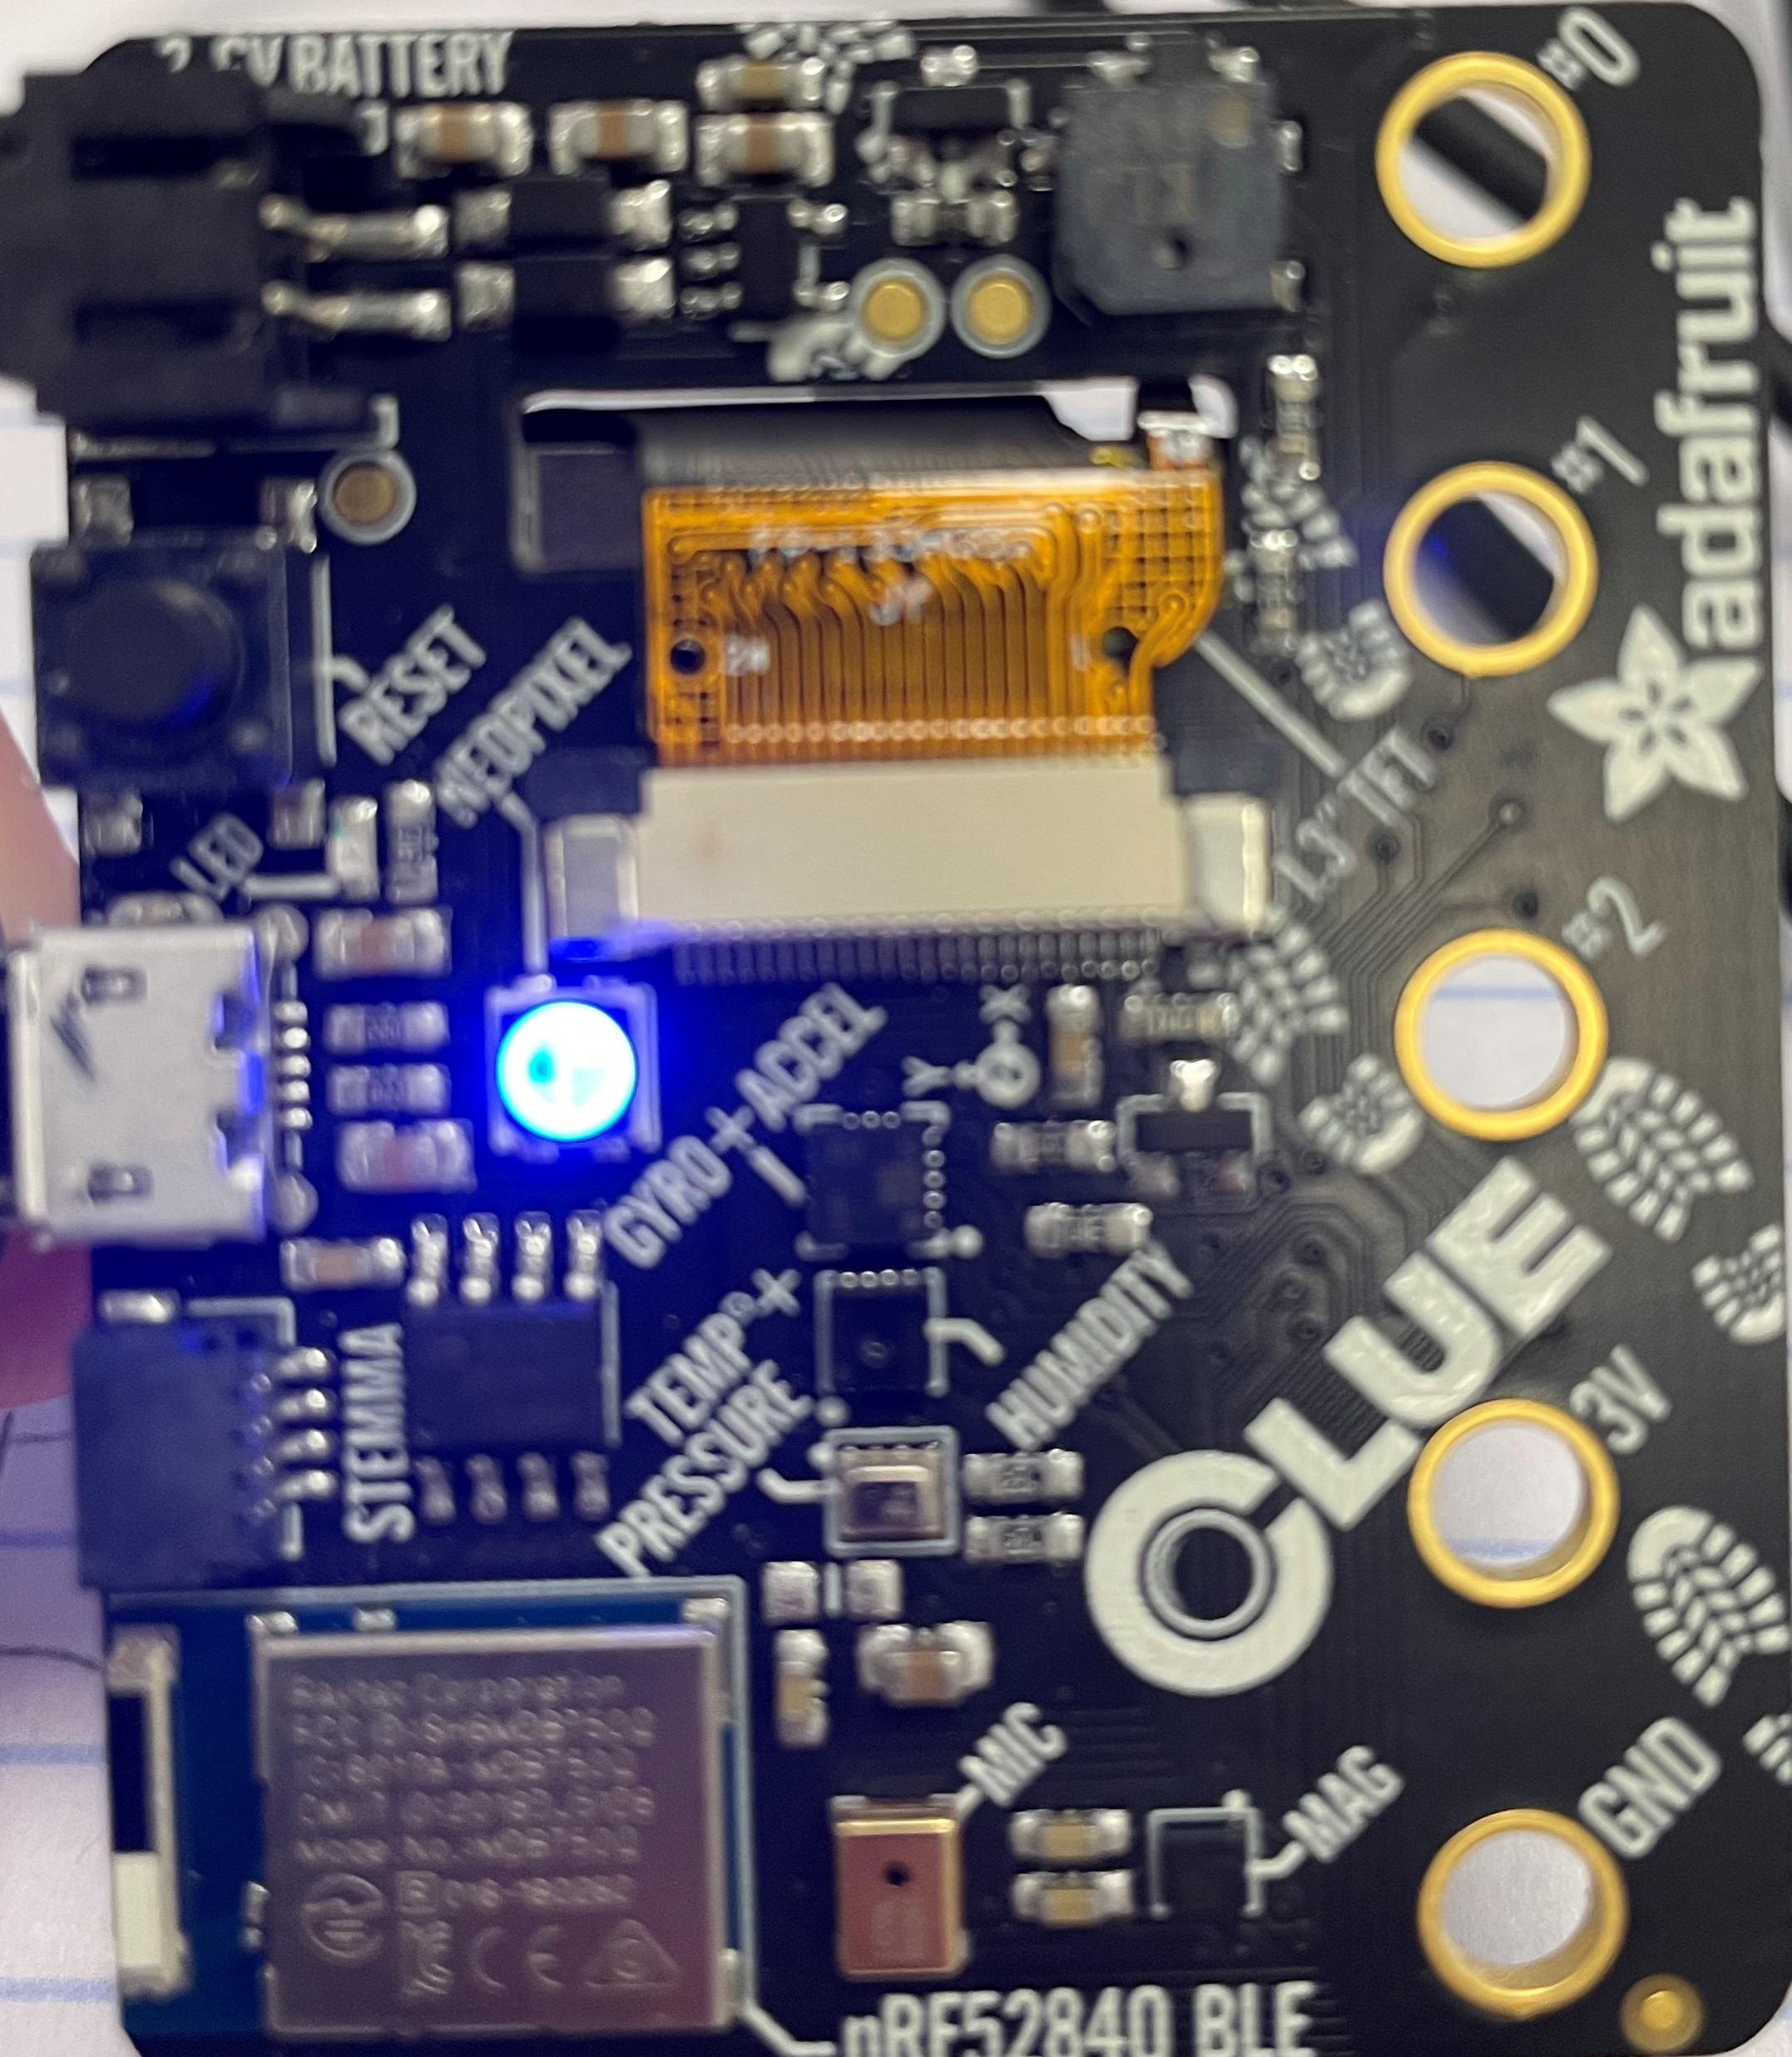
\includegraphics[width=4.5in]{blue.jpg}
\caption{The blue LED displays successful connection to the board}
\label{fig:blue}
\end{figure}

\begin{figure}[H]
\centering
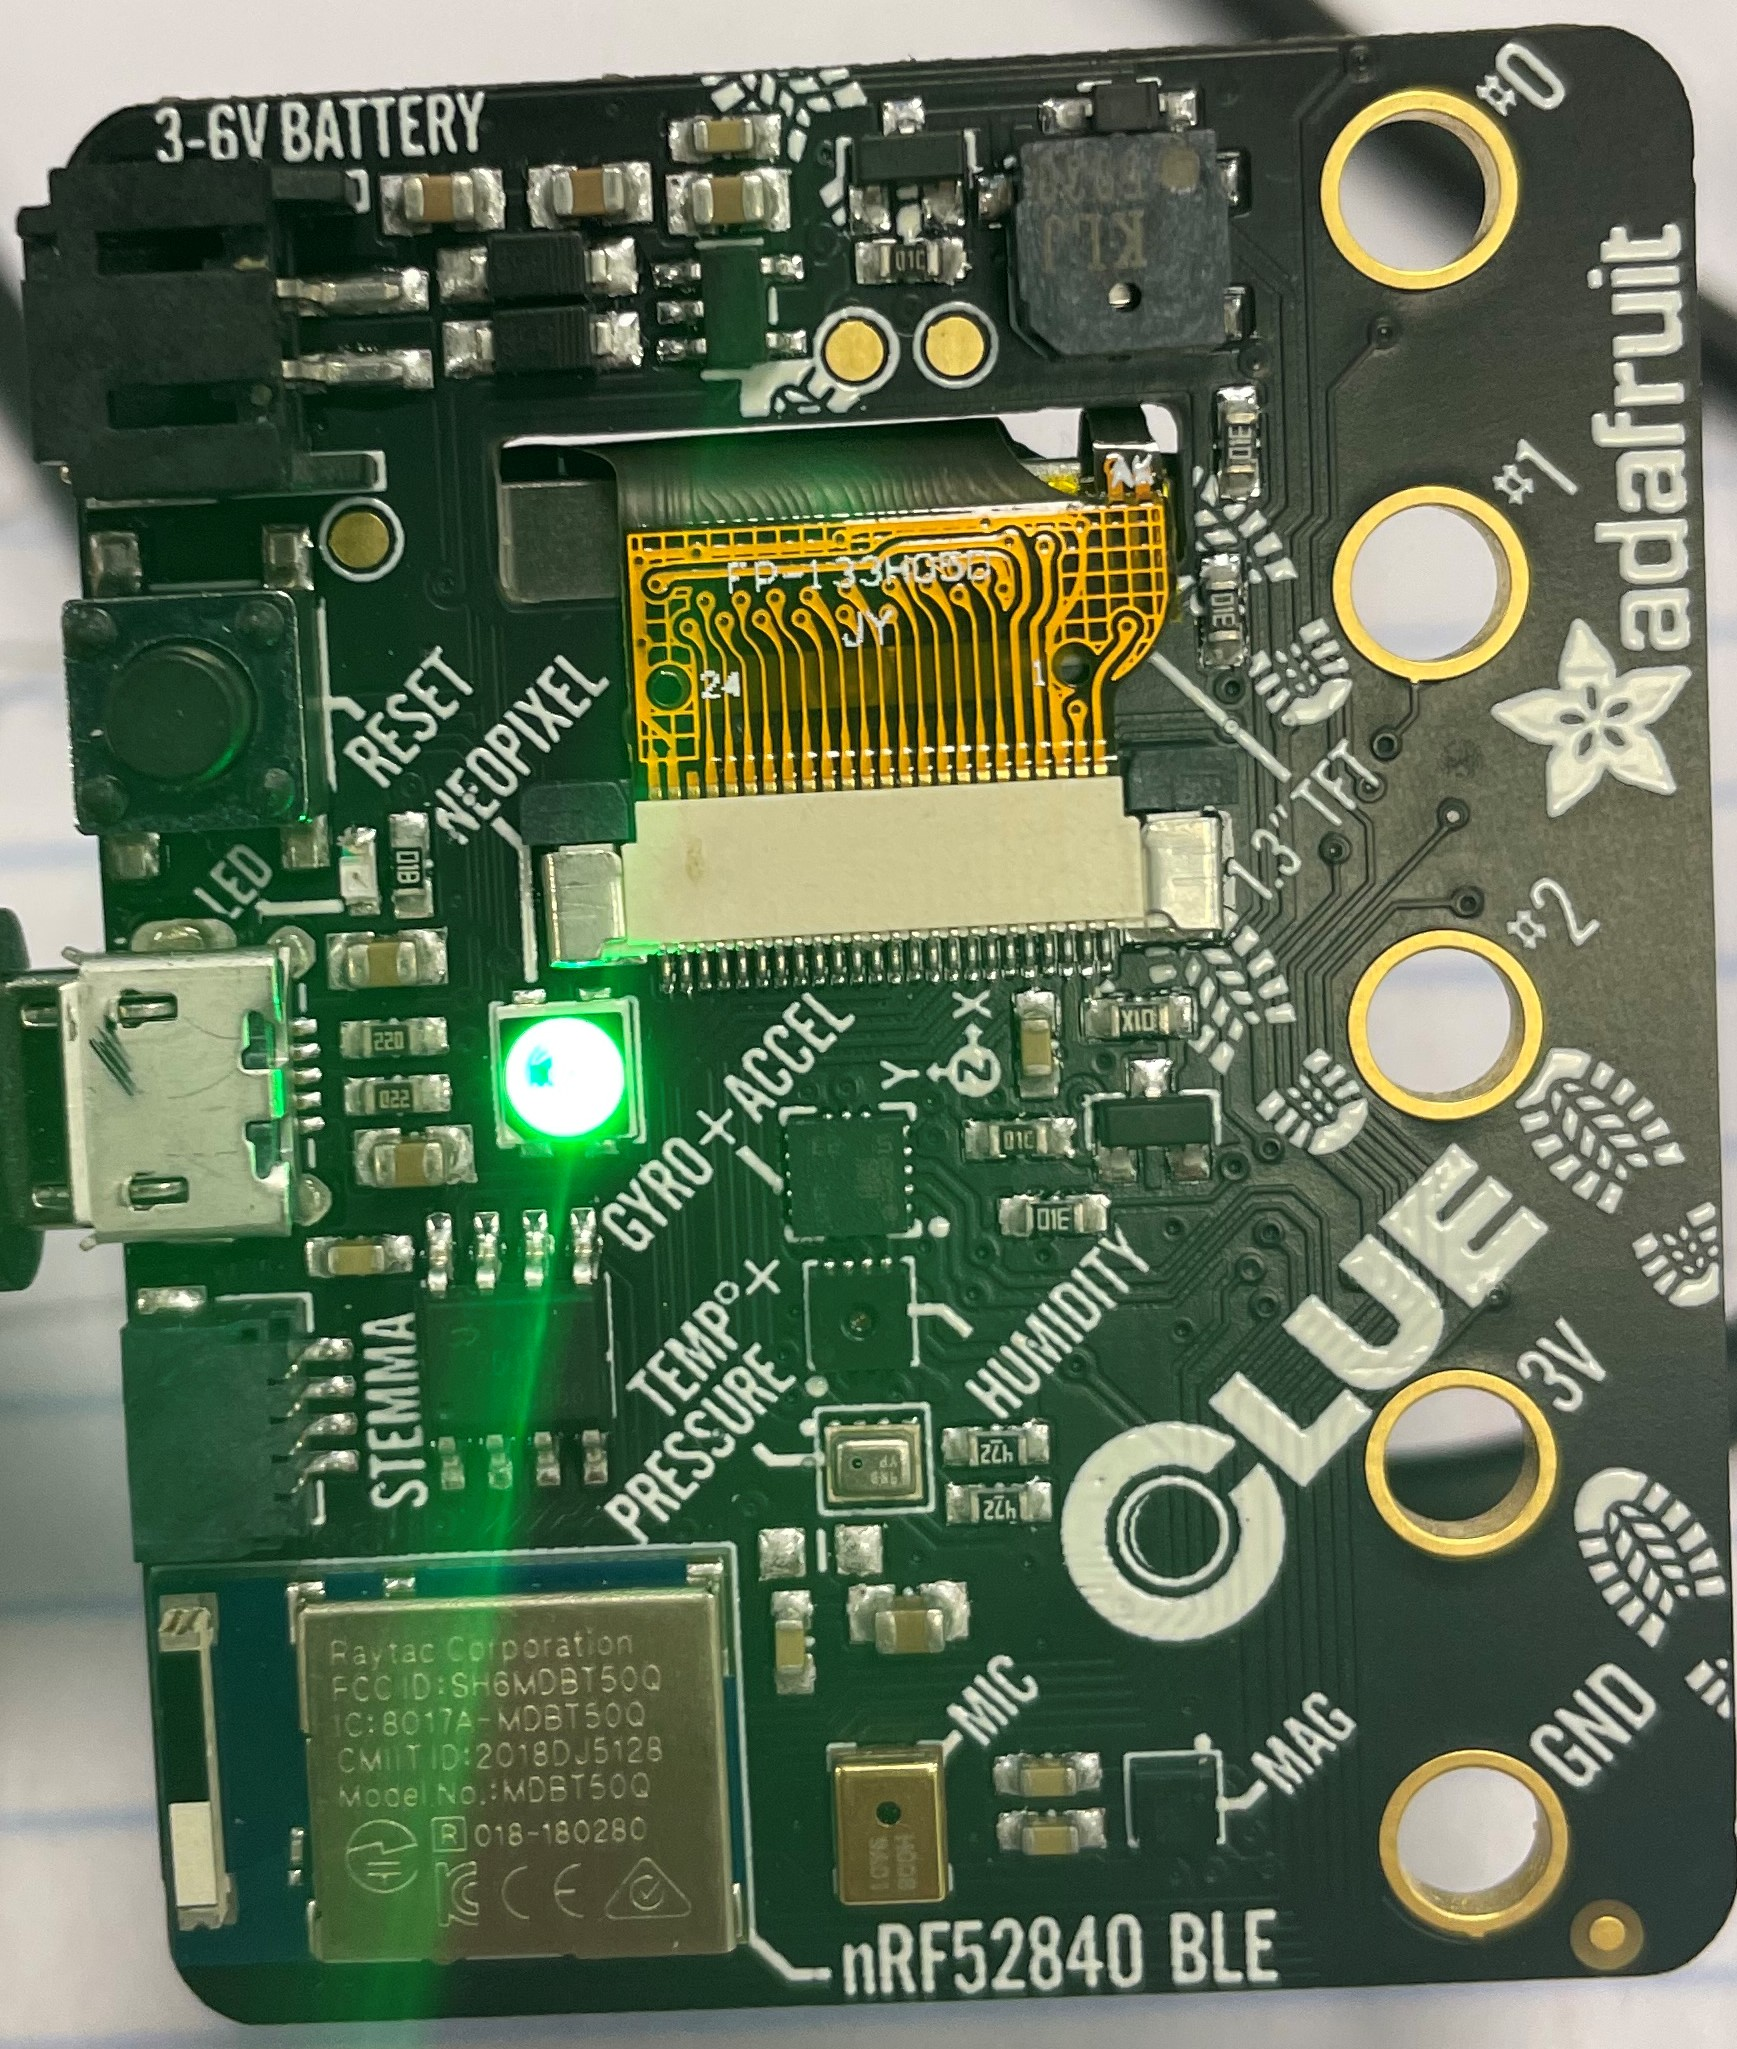
\includegraphics[width=4.5in]{green.jpg}
\caption{The green LED displays user verified on the board}
\label{fig:green}
\end{figure}

\begin{figure}[H]
\centering
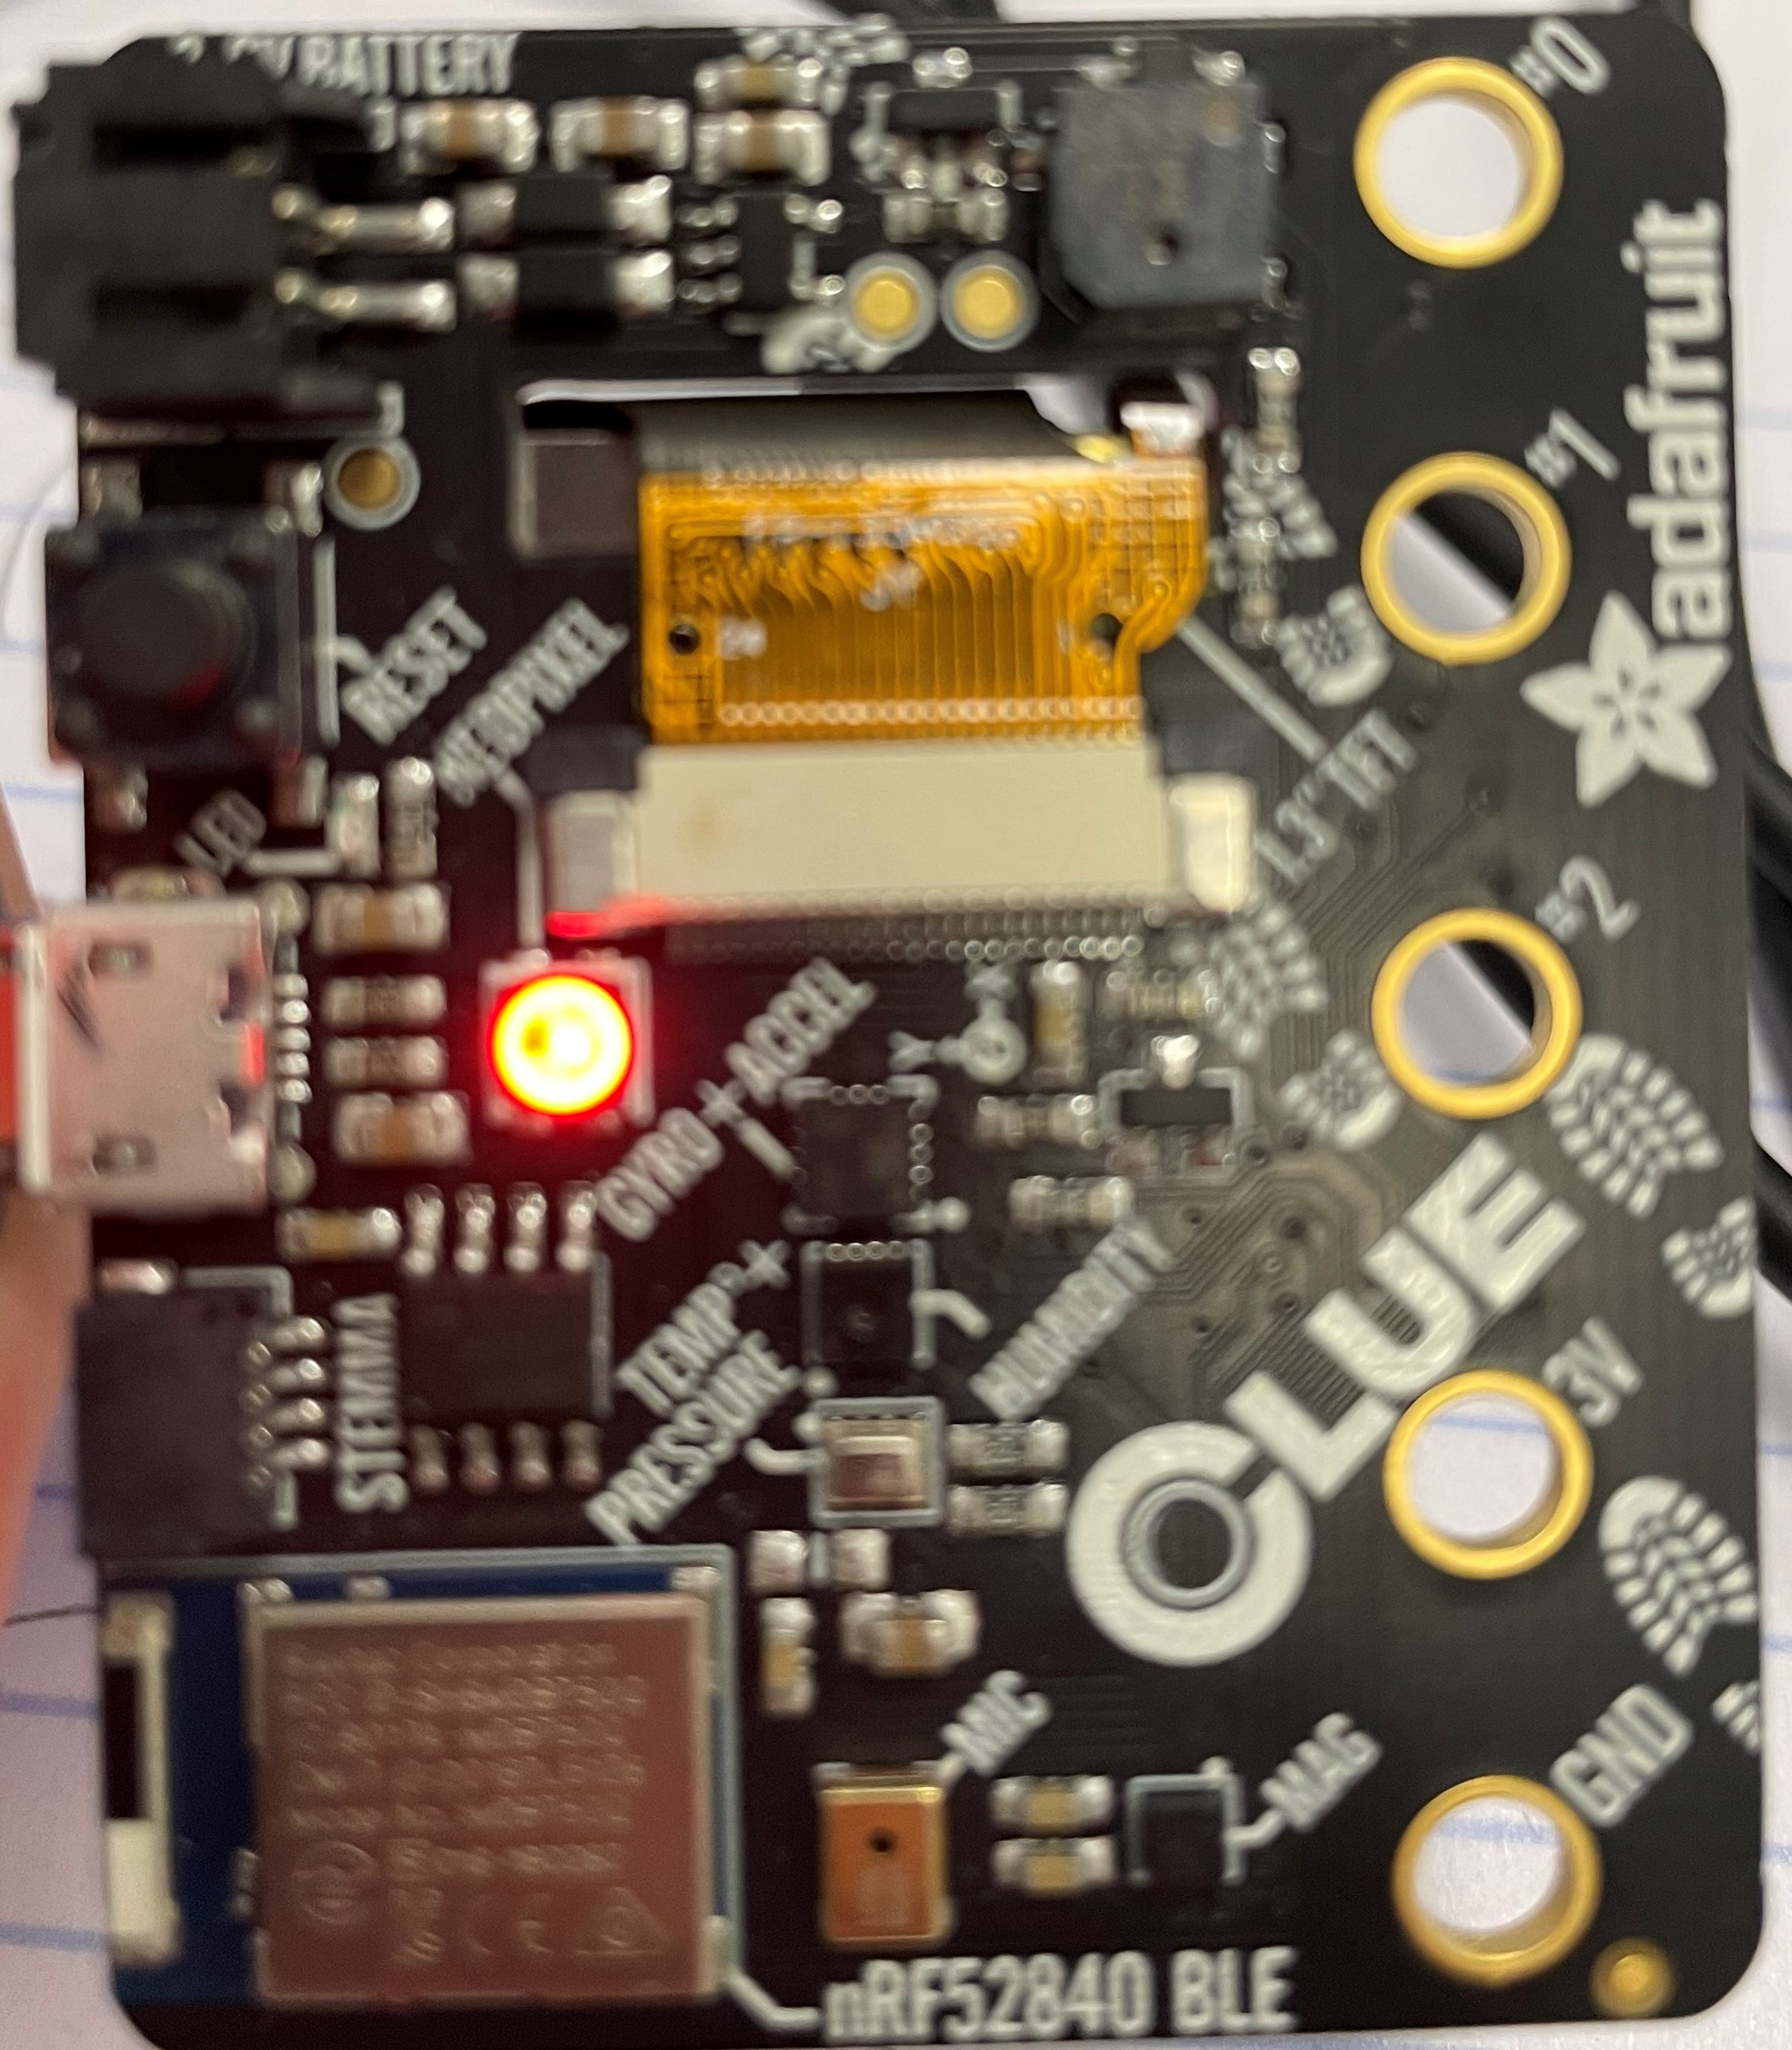
\includegraphics[width=4.5in]{red.jpg}
\caption{The red LED displays the user has used all their attempts}
\label{fig:red}
\end{figure}

\hspace{1cm}\textbf{Figure 1} shows what the user will see on the board if connection between the phone i.e. central device and Bluetooth device i.e. peripheral is successful. If the user has accessed the password manager interface is successfully, the board will display a constant green light, as shown in \textbf{Figure 2}. If the user fails to enter the right (master) password after three times, the device will display a red light (\textbf{Figure 3}), and the user will have to disconnect and re-connect into the Bluetooth device to attempt access to the password manager again. 

\subsection{High Voltage Password Manager Interface}

\begin{figure}[H]
\centering
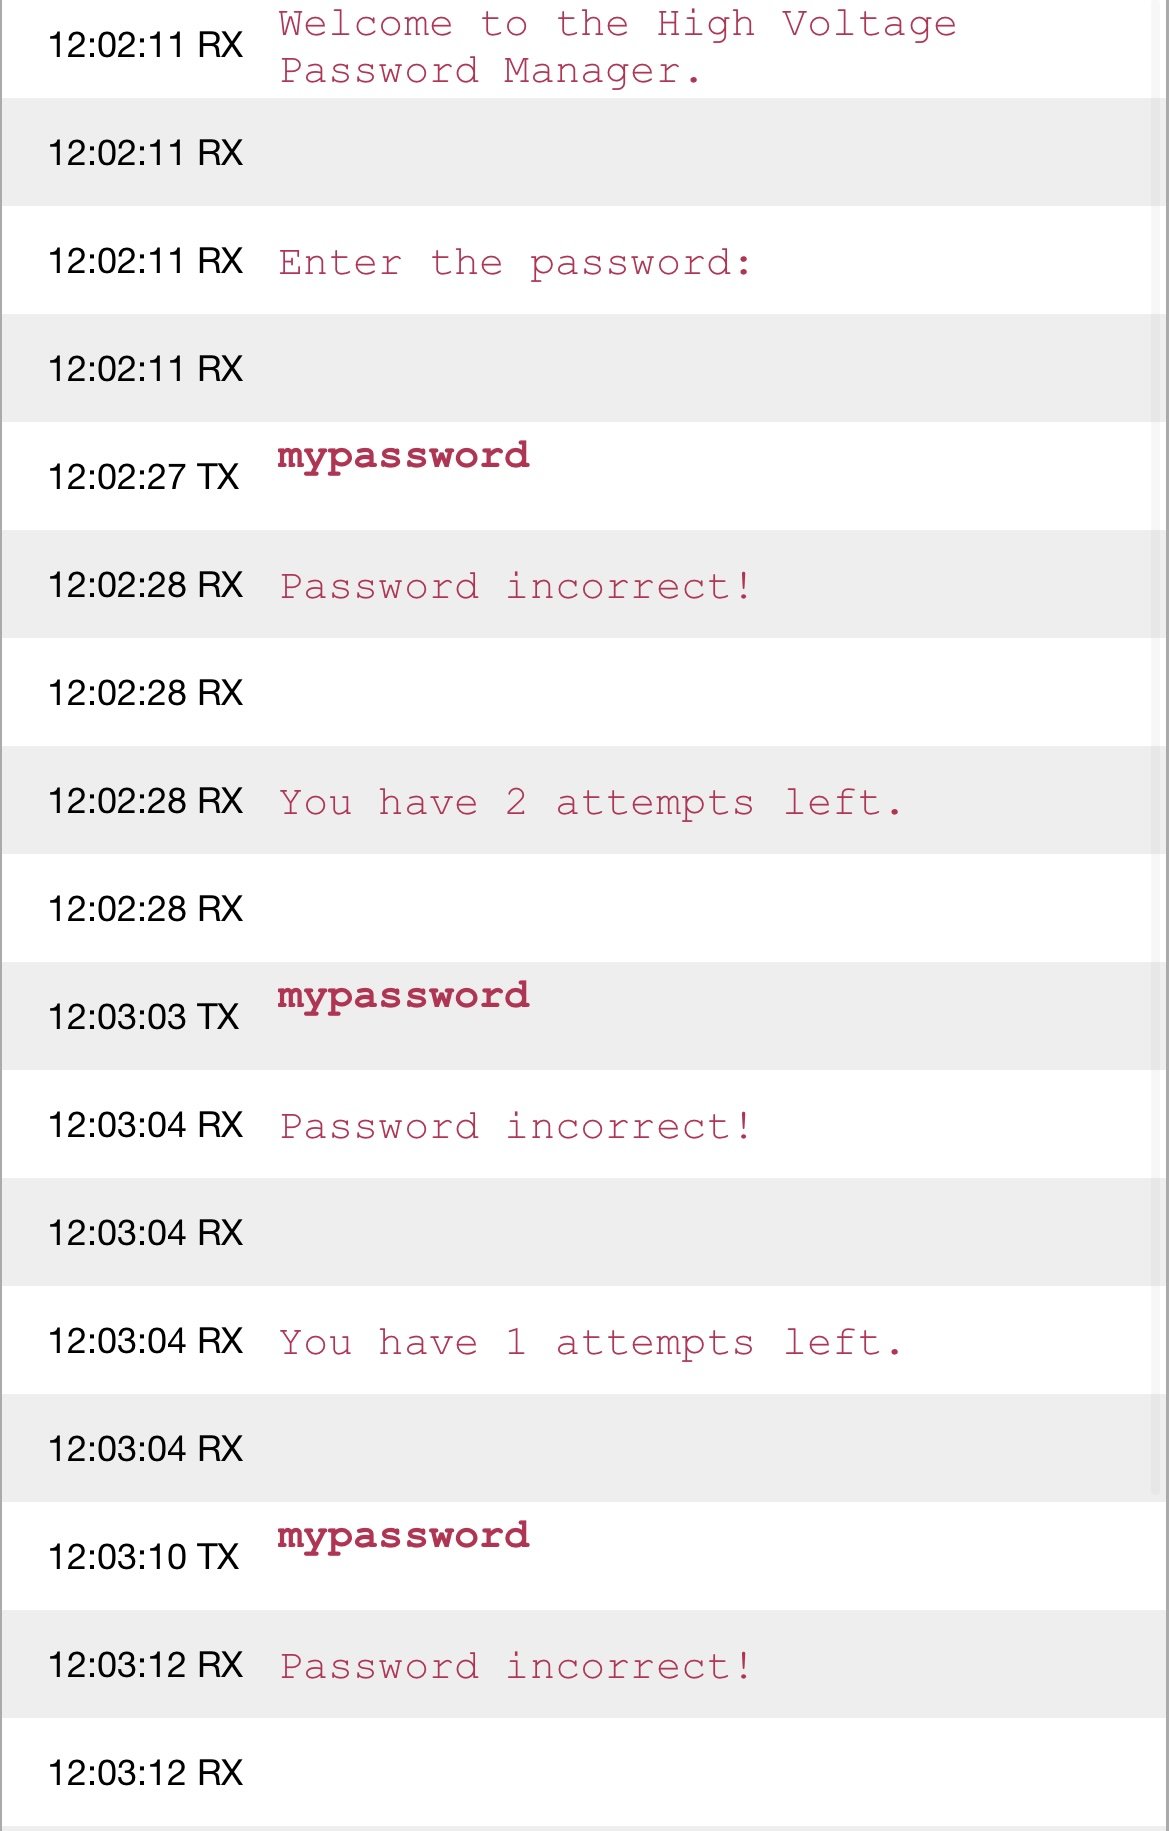
\includegraphics[width=3.7in]{IMG_2450.jpg}
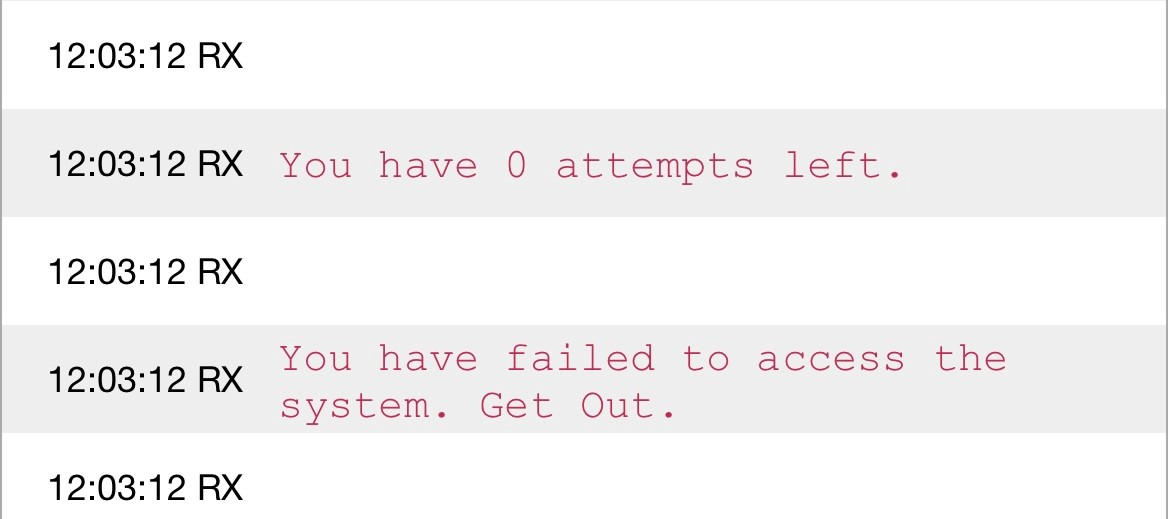
\includegraphics[width=3.7in]{IMG_2451.jpg}
\caption{Password manager with incorrect guess of user password}
\label{fig:fail}
\end{figure}


\begin{figure}[H]
\centering
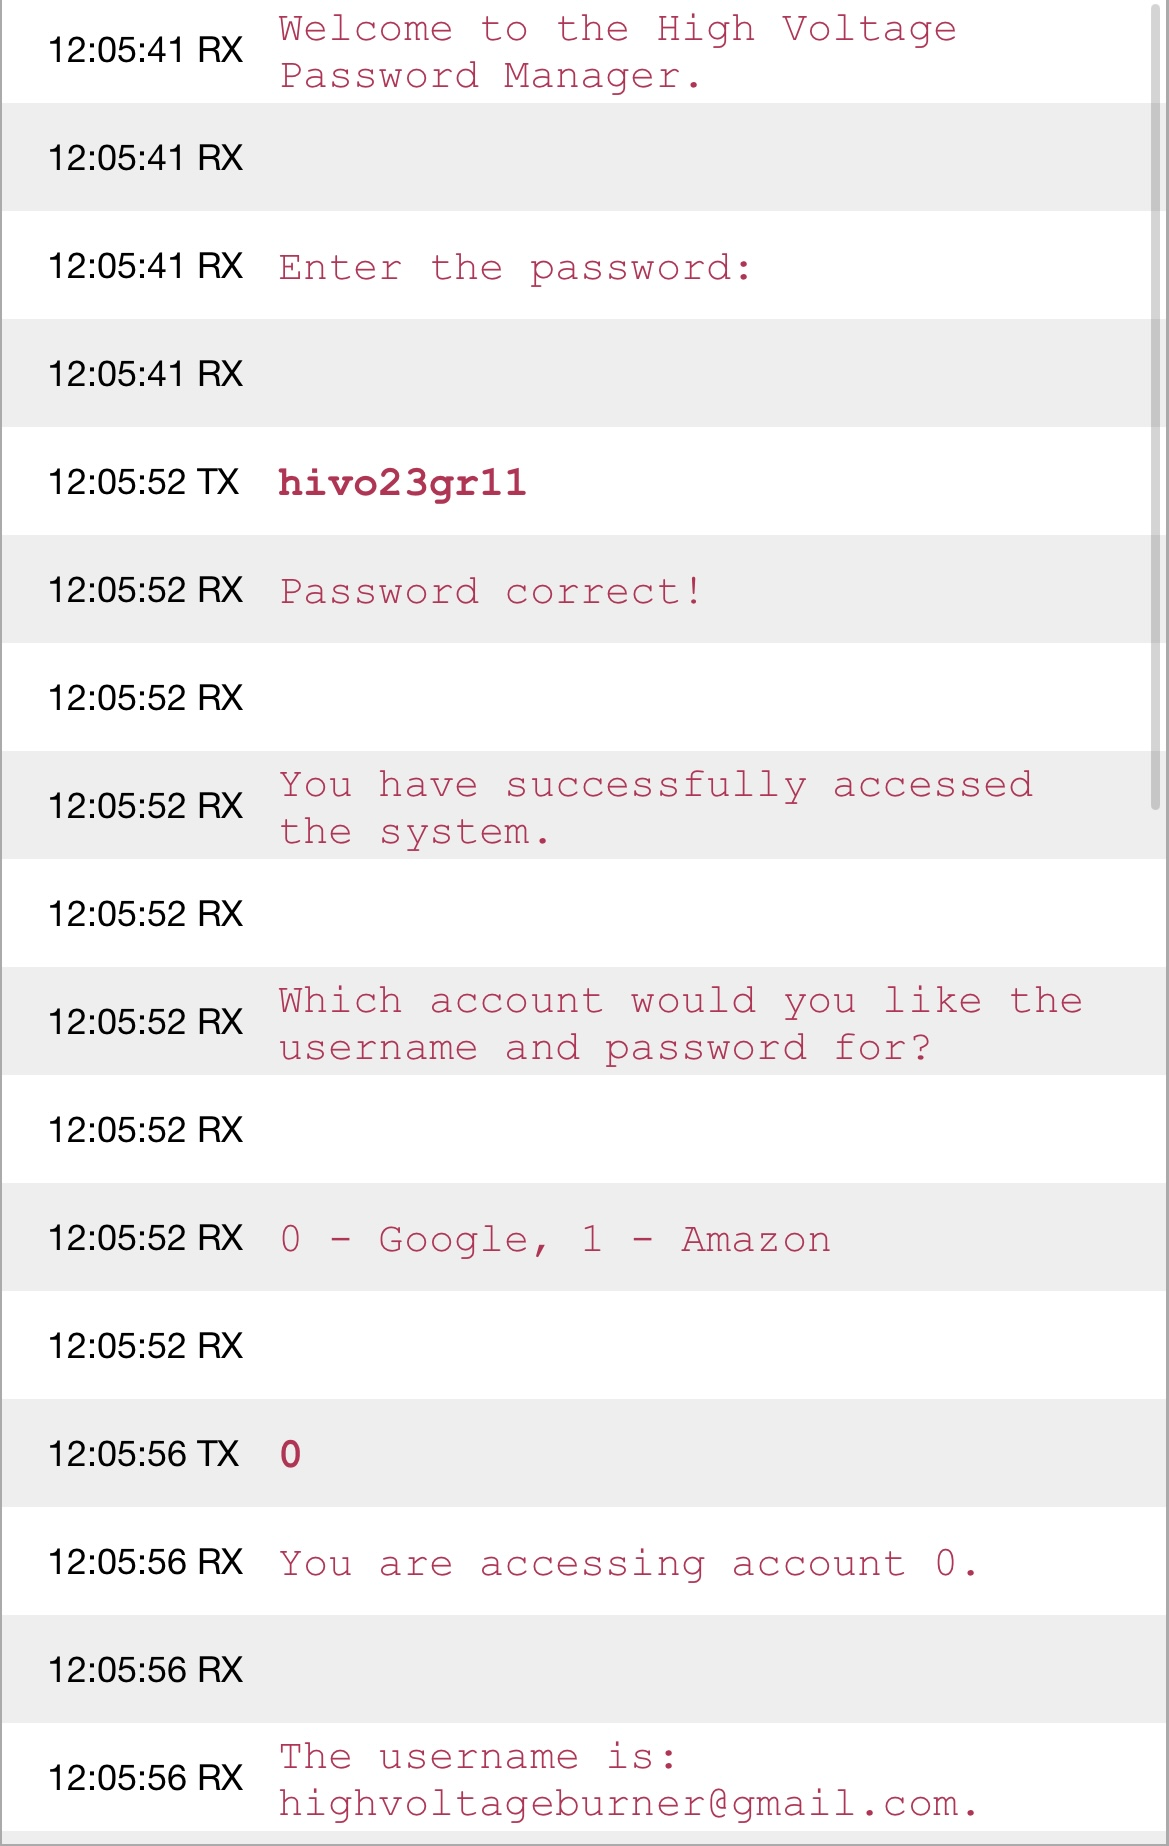
\includegraphics[width=3.7in]{IMG_2453.jpg}

\end{figure}
\begin{figure}[H]
\centering
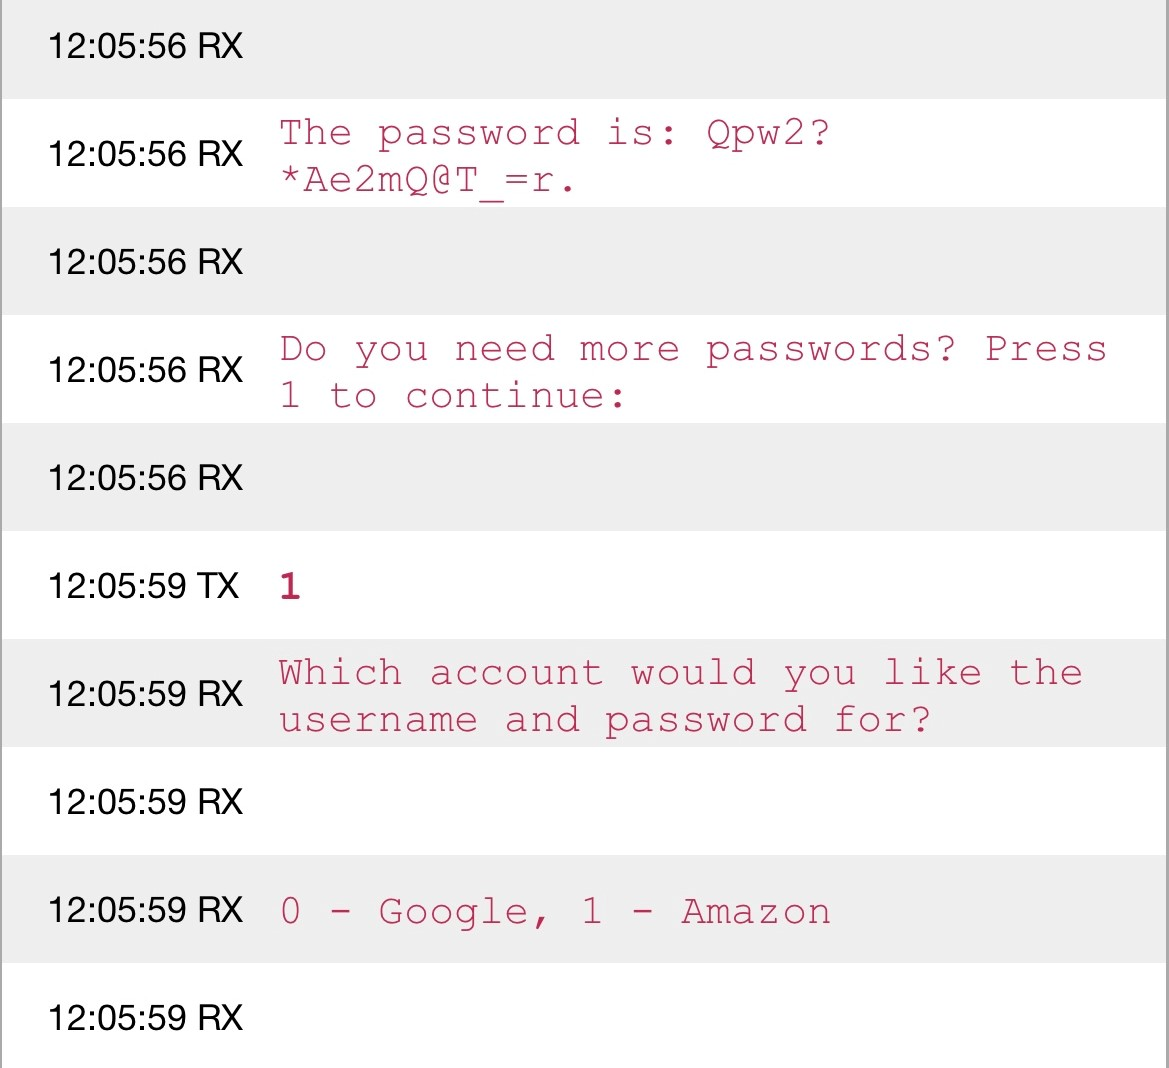
\includegraphics[width=3.7in]{IMG_2454.jpg}
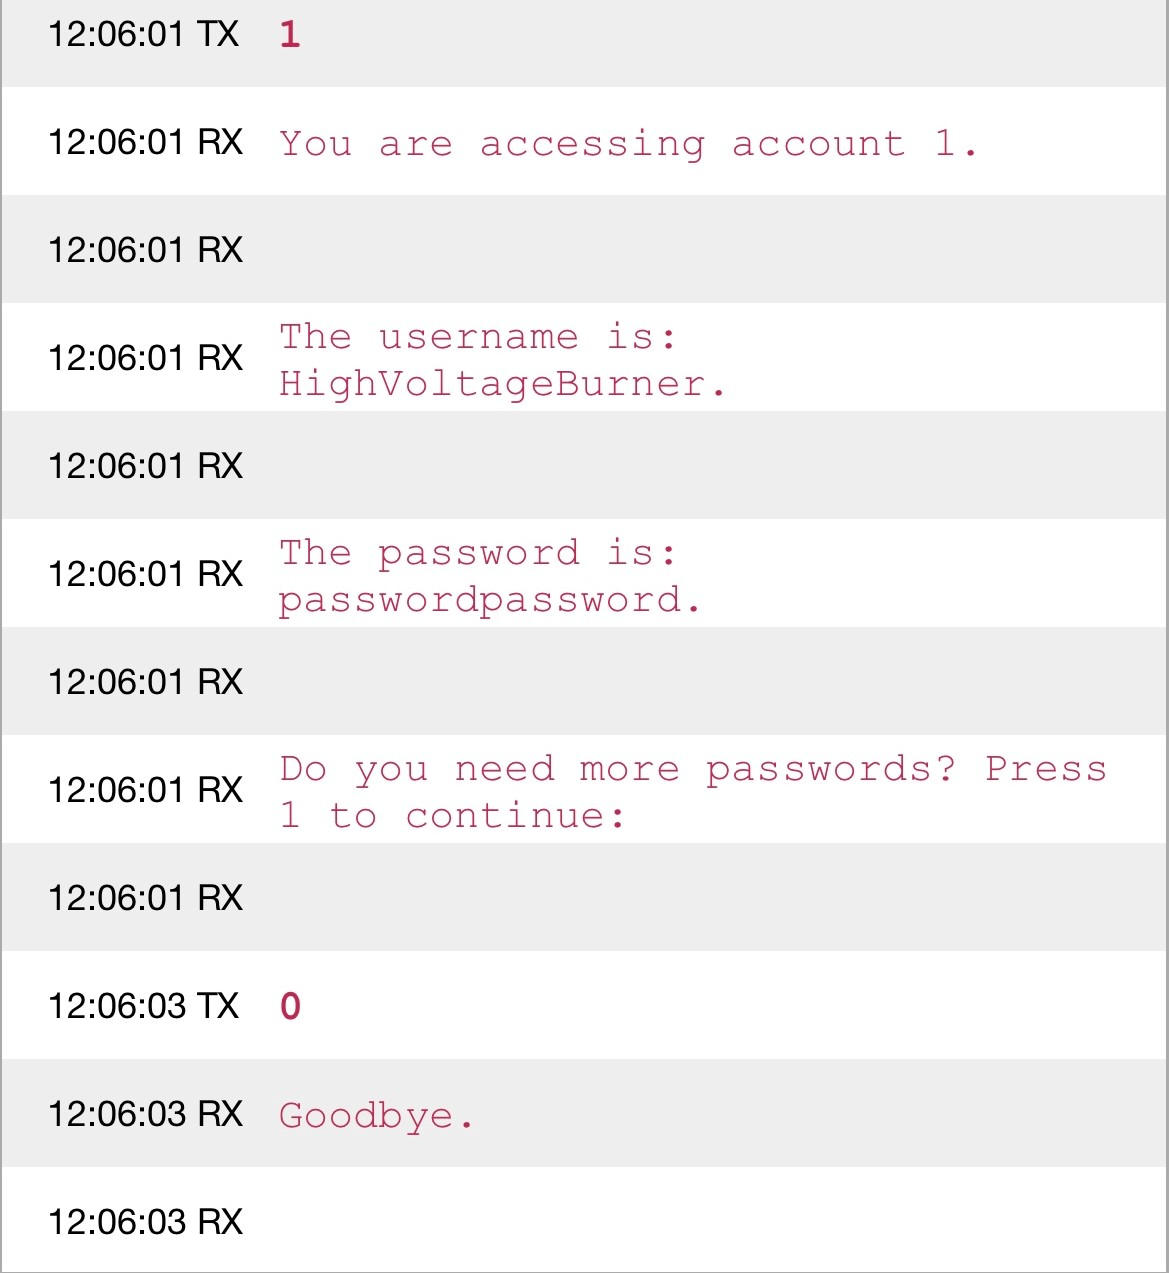
\includegraphics[width=3.7in]{IMG_2455.jpg}
\caption{Password manager with success guess of user password}
\label{fig:success}
\end{figure} 

\hspace{1cm}\textbf{Figure 4} depicts the password manager application interface once the user successfully pairs and connects to the Bluetooth device. The figure displays what interface the user will be able to interact with once they connect into the UART terminal in the Bluefruit Connect phone App.\textbf{Figure 4} displays the text the user will see if they fail to input their master password correctly after three attempts, making them reset to restart the process to access the password manager.\par

\hspace{1cm}If the user successfully enters their password to the password manager, the user will be prompted to search for the account information they want access to. The account information is stored within a designated character array, which allows the user to index through to find what they need, as shown in \textbf{Figure 5}. In \textbf{Figure 5}, the user will either enter the number 0 for their username and password to their google account or 1 for their amazon account information. After the user has acquired the appropriate account information, they will be asked if they want to access other account information stored within the character arrays. If not, they can enter any character to exit the password manager, displaying a goodbye message once they are done. 

\subsection{GitHub Repository}
\url{https://github.com/MihirModi17/High-Voltage_Project}

\section{FUTURE WORK}

\hspace{1cm}If High Voltage were to continue this project, the team would make it so that passwords were read out of a file instead of an array. This would add much more complexity for the programmer, but would allow users to add or delete passwords using this program, leading to a much friendlier user interface. In addition, the team would also need to improve the security (and hence complexity), of the encrypt and decrypt functions. Since the encryption is more complicated, it would take longer to run; when combined with the fact that most of the hardware included on the Adafruit Clue board is not being actively used, it would suit the team's mission goals to design hardware with a more powerful CPU and a smaller form factor.

\section{CONCLUSION}

This project helped everyone on the team improve communication skills and teamwork skills, while teaching the group how to work with GitHub and how to go about working with embedded programming using basic verification testing. Using these skills, the team was able to successfully complete this project. The password manager High Voltage designed helped to teach the group and the AerE 361 class about the importance of an offline password manager and the flaws inherently associated with online password managers, even though it seems that they are very secure. 

\newpage


\bibliographystyle{plain}
\bibliography{ref}
\newpage
\appendix

\section{SOURCE CODE}
\lstinputlisting[label={code:main}, caption={Main Code},language=Arduino]{src/prototypeV3.ino}
\newpage
\lstinputlisting[label={code:helper}, caption={Encryption Helper Code},language=Arduino]{src/encryptionHelper.ino}

\end{document}
